\section{Internet das coisas}
\label{sec:iot}
A Internet nesta última década tem contribuído de forma significativa na economia e sociedade, deixando como legado uma notável infraestrutura de rede de comunicação. O seu maior disseminador nesse período, vem sendo \textit{World Wide Web}(WWW), o qual permite o compartilhamento de informação e mídia de forma global\cite{Chandrakanth:2014}.

No âmbito da economia, por exemplo, o E-Commerce permitiu potencializar as vendas de produtos e serviços, com um faturamento estimado para o ano de 2016 de aproximadamente 56,8 bilhões de reais no Brasil, segundo ecommercenews\footnotemark \footnotetext{https://ecommercenews.com.br/noticias/pesquisas-noticias/e-commerce-brasileiro-deve-crescer-18-e-faturar-r-568-bilhoes-em-2016}. Além do benefício direto para sociedade provindo do E-Commerce, onde as pessoas podem realizar pesquisa de preços de serviços e produtos e, adquiri-los de forma comoda, sem precisar se deslocar até um ponto de venda, a Internet dispõe para a sociedade diversas outras oportunidades, como cursos a distância oferecidos por diversas universidades de todo o mundo, a exemplo dos cursos disponibilizados pela plataforma Coursera\footnotemark \footnotetext{\url{https://pt.coursera.org/}}. 

A Internet está se tornando cada vez mais persistente no cotidiano, devido, por exemplo, ao crescente número de usuários de dispositivos móveis, os quais possuem tecnologias de conexão com a Internet, as quais cada dia tornam-se mais acessíveis (presentes em locais que não tinham e, mais baratas)\cite{Chandrakanth:2014}.

Em 2010 havia aproximadamente 1,5 bilhão de PCs conectados a Internet e mais que 1 bilhão de telefones móveis\cite{Sundmaeker:2010}. Segundo Gartner\footnotemark \footnotetext{\url{http://www.gartner.com/newsroom/id/3165317}}, 6,4 bilhões de coisas estarão conectadas até o final de 2016 e, em 2020 esse número atingirá cerca de 20,8 bilhões. A previsão de \cite{Sundmaeker:2010}, a qual dizia que a denominada Internet dos PCs seria movida para o que se chama de Internet das Coisas fica então mais evidente neste atual cenário.

A ideia básica da \textit{Internet of things (IoT)}, traduzido para o português como Internet das Coisas é a presença pervasiva de uma variedade de "coisas ou objetos", tais como RFID tags, sensores, telefones móveis, dentre outros. Os quais, através de esquemas de endereçamento único são capazes de interagir com os outros e cooperar com seus vizinhos para alcançar um objetivo em comum\cite{Atzori:2010}. Outros exemplos de "coisas ou objetos" podem ser pessoas, geladeiras, televisores, veículos, roupas, medicações, livros, passaportes, contanto que possam ser identificadas unicamente e possam se comunicar com as outras coisas e/ou possam ser acessados remotamente por humanos.

Dentre as diversas definições de Iot pode-se citar duas, a primeira define de maneira mais geral, tanto a atual realidade, quanto a prospeção futura. Já a segunda especifica melhor como deve ser o cenário ideal da Internet das Coisas, pois já embuti explicitamente os conceitos de capacidades de autoconfiguração, interoperabilidade e interfaces inteligentes.
\begin{enumerate}
\item Segundo\cite{iot2020:2008}, \textit{Internet of Things} significa rede mundial de objetos unicamente endereçáveis e interconectados, seguindo os protocolos dos padrões de comunicação.
\item IoT é parte integrante da futura Internet e pode ser definida como uma infraestrutura de rede global dinâmica com capacidades de autoconfiguração baseada nos padrões e interoperabilidade dos protocolos de comunicação onde coisas físicas e virtuais têm identidade, atributos físicos, personalidade virtual, usam interfaces inteligentes e, são integradas dentro da rede de informações \cite{Sundmaeker:2010}.
\end{enumerate}

Diante deste cenário da IoT, pode-se citar exemplos de aplicações em diversos domínios, tais como, logística e transporte; cuidados com a saúde; ambiente inteligente (casa (seção \ref{sec:hns}), escritório);\cite{Atzori:2010} verificação de procendência alimentícia; dentre outros. Abaixo se tem uma breve descrição de duas aplicações, uma na área de cuidados com a saúde e outra na verificação de procedência de alimentos, respectivamente.

\begin{itemize}
\item Dispositivos implantáveis com capacidade de comunicação sem fio podem ser utilizados para armazenar registros sobre a saúde de um paciente em situações de risco e podem ser decisivos para salvar a vida do paciente. A capacidade de ter acesso a essas informações nessas circunstâncias fazem com que hospitais possam saber de imediato como tratar um paciente que esta a caminho. Esta possibilidade é especialmente útil para pessoas com diabetes, cancer, problemas de coração na arteria coronária, doenças do pulmão, assim como a pessoas com implantes médicos complexos, tais como, marcapassos, tubos, transplantes de orgãos e aqueles que podem ficar inconscientes e incapazes de comunicar-se durante uma operação. \cite{Weber:2010}
\item Rastreabilidade de produtos alimentícios ajudam os usuários a verificar a origem de um produto, assim como informações de composição química, dentre outros. Mas também previne de doenças não desejadas. Por exemplo, avisos atuais sobre a mercadoria em questão podem ser disponibilizados à medida que o produto sai da origem e vai passando para os outros níveis de consumo, desta forma os consumidores podem evitar o contágio de doenças como gripe aviária e,  encefalopatia espongiforme bovina (EEB), mais conhecida como doença da vaca louca.\cite{Weber:2010}
\end{itemize}

Apesar da grande potencialidade da visão da Internet das Coisas, a qual gerou em 2015 um faturamento em torno de 130,33 bilhões de dolares americanos e tem prospeção de chegar até 883.55 bilhões em 2020\footnotemark \footnotetext{http://www.marketsandmarkets.com/Market-Reports/iot-application-technology-market-258239167.html}, ainda existem muitos desafios a serem vencidos, tais como segurança da informação, armazenamento e processamento de grande quantidade de dados, dentre outros. Adentrando um pouco em um dos desafios da IoT, o da disponibilidade de uma interface de comunicação (acesso aos serviços e informações dos dispositivos) e programação comum aos objetos, pode-se dizer que a falta desta padronização faz com que se torne oneroso o desenvolvimento de aplicações para o objeto, pois cada coisa possui suas próprias interfaces, logo para cada dispositivo um desenvolvimento a parte. Mais difícil ainda é prover uma única funcionalidade ou serviço com a composição dos diversos objetos. Para diminuir a dificuldade deste cenário, pode-se disponibilizar os dispositivos como serviços WEB (seção \ref{subsec:dispositivosweb}), assim sendo pode-se utilizar os protocolos WEB como linguagem comum de integração dos dispositivos a Internet.\cite{Franca:2011}

\subsection{Serviços web}
Segundo\cite{Dustdar:2005}, um serviço web é um sistema identificado por uma URL\footnotemark \footnotetext{Acrônimo para Uniform Resource Locator e é uma referência (um endereço) para um recurso na Internet.\cite{oracle:url}}, no qual suas interfaces públicas são definidas e descritas usando XML\footnotemark \footnotetext{Extensible Markup Language (XML) é uma simples e flexível linguagem de marcação utilizada para codificar documentos através de regras produzidas por humanos, as quais podem ser manipulados (compreendidas) por máquinas \cite{w3c:xml}\cite{w3c:xmlschema}} e, suas definições podem ser descobertas por outros sistemas. Sistemas então podem interagir com os serviços web utilizando suas definições e descrições. Através destas utiliza-se mensagens XML que são trasmitidas seguindo os protocolos padrão (definidos por W3C\footnotemark \footnotetext{\url{https://www.w3.org/}}) da Internet para que haja tal interação.

Serviços web surgiram tendo como principal foco o reuso de aplicações existentes (dentre as quais incluiam código fonte legado) para que pudessem se integrar de forma leve com outras aplicações, geralmente essa integração tinha como referência o desejo de  novas formas de compartilhamento dos serviços ao longo das diversas linhas do negócio ou entre parceiros. Para melhor enteder o proposito dos serviços web, considere, como exemplo, uma companhia de seguros que decidiu oferecer um serviço de cotação on-line. Então ao invés de desenvolver toda a aplicação do inicio, a empresa utiliza-se do serviço web de outra empresa(epecializada em cálculos de seguro). Este serviço pode, por exemplo, oferecer um formulário de cotação e, após o cliente informar os dados necessários, o serviço web apresentará uma cotação baseado nos dados informados. Além disso, caso o cliente escolher comprar tal seguro, pode-se ainda utilizar de outro serviço web, oferecido por uma outra empresa, o qual irá processar o pagamento de acordo com os dados passados para ele e então retorna o resultado do processamento para o cliente e para a empresa original(que desejou construir o serviço de cotação on-line)\cite{Papazoglou:2008}. O cenário da Figura \ref{fig:ws_purchase_order} demonstra um outro exemplo de uso de diferentes serviços para prover um único serviço, o de um pedido de uma ou mais mercadorias, ambiente comum do E-Commerce. 

\begin{figure}[!htb] \centering 
  \centering
  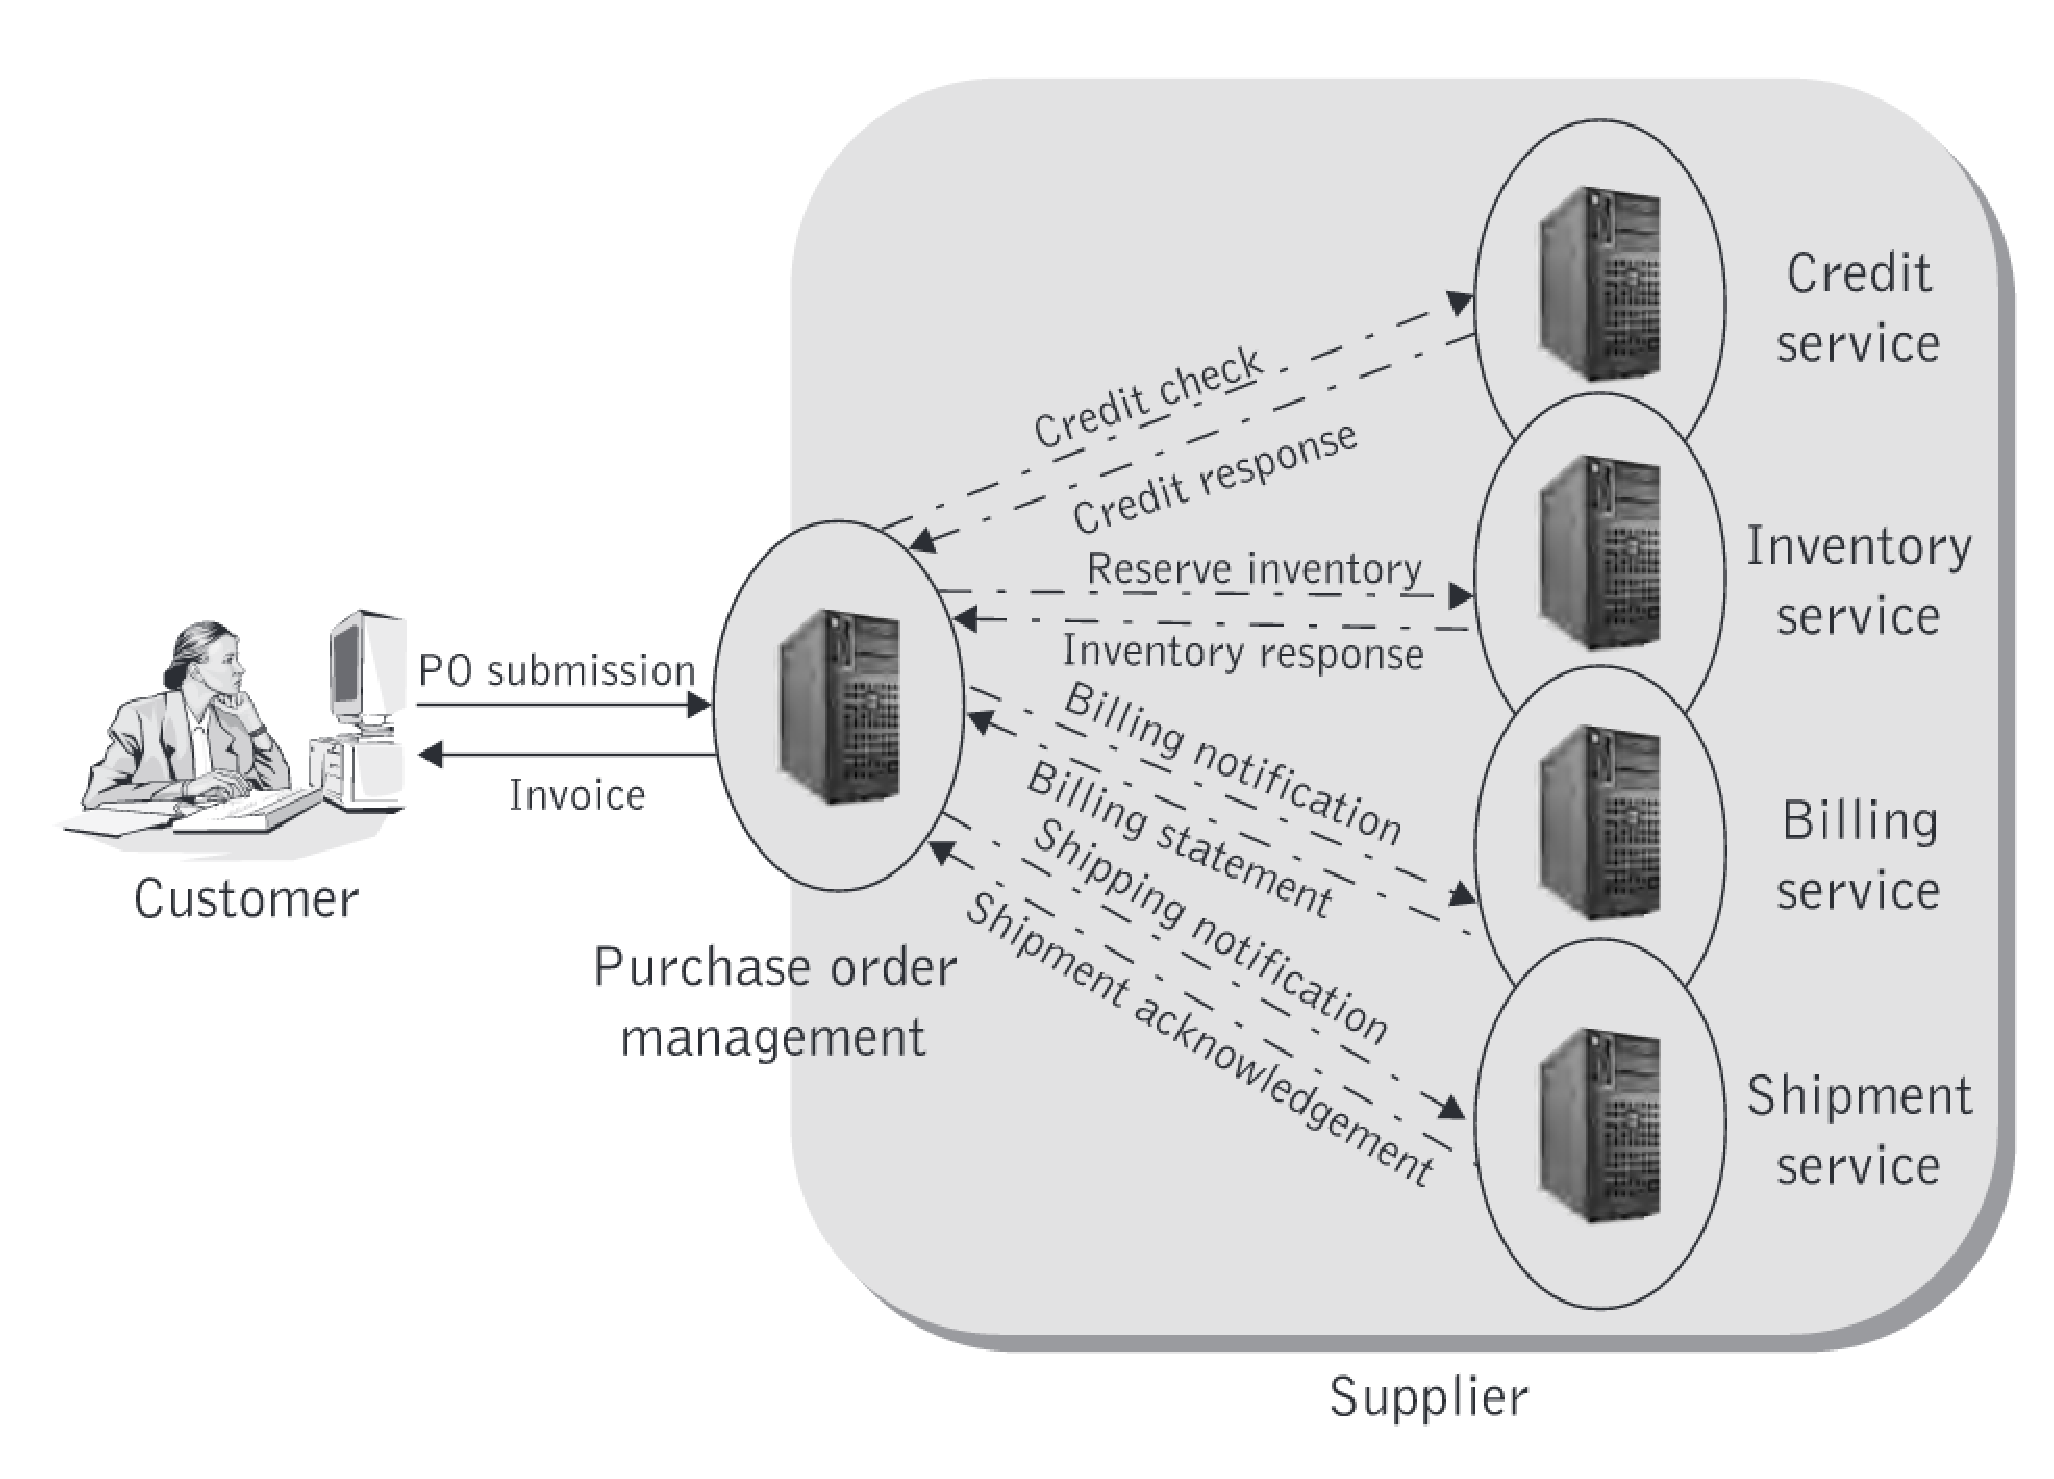
\includegraphics[width=0.8\columnwidth]{fundamentacao/webservice_purchase_order} 
  \caption{Utilização de diferentes serviços web para prover o serviço de pedido de um E-Commerce.\cite{Papazoglou:2008}} 
  \label{fig:ws_purchase_order}
\end{figure}

O cenário do serviço(Figura \ref{fig:ws_purchase_order}) pode ser descrito da seguinte forma:
\begin{enumerate}
\item \textit{Consumer}(Consumidor) escolhe seu(s) produto(s), informa dados do cartão de crédito e outras informações necessárias e, clica no botão comprar. Requisição é enviada ao \textit{Purchase order management}(Gerenciador de pedidos de compra).
\item O gerenciador então verifica se o cartão do cliente tem crédito suficiente através da funcionalidade \textit{Credit check} do serviço \textit{Credit Service} e, o serviço da uma resposta.
\item Gerenciador capta a resposta e, caso cliente tenha crédito suficiente, inicia o processo de reserva do pedido através da funcionalidade textit{Reserve inventory} do serviço \textit{Invetory service}.
\item Gerenciador capta resposta \textit{Inventory response}, caso o pedido tenha sido reservado com êxito, o gerenciador utiliza o \textit{Billing service} para processar o pagamento.
\item \textit{Billing service} retorna o estado do pagamento, se pagamento foi processado com êxito o gerenciador utiliza agora a funcionalidade \textit{Shipping notification} do serviço \textit{Shipment service} para prover o serviço de entrega.
\item Gerenciador recebe a resposta \textit{Shipment acknowledgement} e informa ao cliente (\textit{Invoice}) a data prevista para entrega do(s) produto(s) do cliente.
\end{enumerate}

No cenário apresentado anteriormente há uma ressalva que deve ser feita, a qual dita uma das características de um serviço web (serviço assícrono ou sícrono, descrito logo a seguir), no item 5, por exemplo, o pagamento pode demorar mais de um dia para concluir seu processamento, então o cliente poderia receber um retorno do sistema do tipo, pagamento aguardando processamento, ou seja, a resposta do processamento do pagamento(realizado ou não realizado), poderia vir através de um envio de email ou SMS, somente depois de muito tempo.

Serviços web possuem algumas características que se fazem importantes saber:
\begin{enumerate}
\item Podem ser ditos \textit{stateless} (sem estado) ou \textit{stateful} (com estado). Se um serviço pode ser invocado repetidamente sem ter que manter um contexto ou estado este é denominado textit{stateless}. Como exemplo de serviço textit{stateless} pode-se citar a recuperação de informação de um sensor de temperatura, pois não precisa de nenhum tipo de memória para manter o que aconteceu durante as requisições ao serviço. Já os serviços que precisam manter seus contextos preservados de uma invocação para a próxima requisição, estes são \textit{stateful}. Por exemplo, um usuário quando chama um serviço (Levar compras) de um textit{Home Network Service} (ver seção \ref{sec:hns}), este então começa sua execução: um veículo( um serviço) leva a carga até uma determinada área próxima ao elevador(um serviço) e, uma garra mecânica (um serviço) pega a carga e coloca dentro do elevador. Observe que o serviço Levar compras é a composição de diferentes serviços e não pode ser chamado e executado diversas vezes continuamente sem a necessidade de manter seu contexto entre os diferentes serviços envolvidos, pois o ambiente não tem mais de um carro, mais de uma garra e elevador. Então a menos que este já tenha terminado toda a sua execução, poderia ser chamado e executado novamente. Por tal motivo este serviço mantêm um estado (em execução ou sem trabalho) o qual depende dos estados dos serviços envolvidos.\cite{Papazoglou:2008}
\item Podem ser ditos com baixo nível de acoplamento (textit{loose coupling}) quando os serviços interagem uns com os outros e utilizam-se as tecnologias padrões da Internet, permitindo dessa forma construir pontes entre sistemas que de outra forma exigiriam grandes esforços de desenvolvimento de software. O termo acoplamento indica o nível de dependência entre serviços.\cite{Papazoglou:2008}
\item Podem ser ditos síncronos e assícronos. Quando síncrono, clientes realizam suas requisições e ficam sempre aguardando uma resposta. O cliente é dependente de tal resposta para continuar sua computação. Se uma operação for incapaz de ser completada, todo o resto da computação é impedida de continuar. Enquanto que nos assícronos o cliente não necessita aguardar uma resposta para continuar a execução de sua aplicação. Quando um cliente invoca um serviço assíncrono, o cliente normalmente envia um documento inteiro, como uma ordem de pagamento ou, uma lista de itens de um carrinho de compra juntamente com o tipo de pagamento e endereço de entrega. O serviço aceita o documento inteiro e processa-o, podendo retornar ou não uma mensagem de resultado. A respota do serviço, se existir alguma, pode acontecer horas ou talvez dias depois.\cite{Papazoglou:2008}
\end{enumerate}

Serviços web possuem baixo nível de acoplamento e utilizam padrões para oferecer suas funcionalidades, pois tais serviços tem a intenção de prover comunicação a diferentes tipos de aplicações, que possivelmente são executadas em diferentes plataformas. A \textit{Web Service Description Language}(WSDL) usa o formato XML para descrever os métodos oferecidos por um serviço web, incluindo parâmetros de entrada e saída, tipos de dados e, protocolo de transporte utilizado (normalmente o HTTP). Além de informações referente ao provedor do serviço, tais como, endereço e contato da empresa desenvolvedora do serviço. O \textit{Simple Object Access Protocol}(SOAP, seção \ref{subsec:soap}) é utilizado para as trocas de mensagens (formatadas em XML) entre as entidades envolvidas no modelo de serviço web citado\cite{Dustdar:2005}, como pode ser visto na Figura \ref{fig:wsmodelsoap} e explicado logo abaixo. Esse tipo de serviço web é chamado de serviço web baseado em SOAP\cite{Belqasmi:2011}.

\begin{figure}[!htb] \centering 
  \centering
  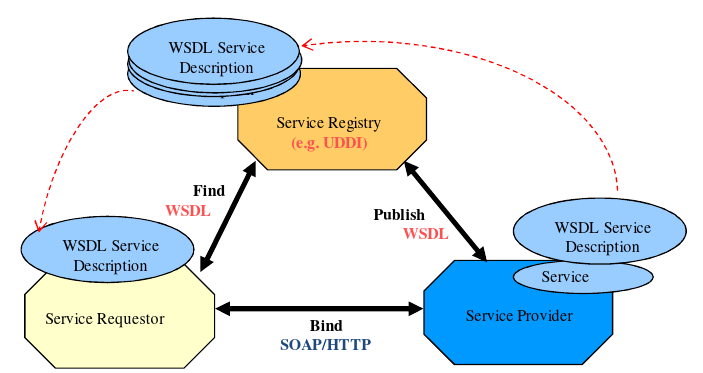
\includegraphics[width=0.8\columnwidth]{fundamentacao/webservice_soap_model} 
  \caption{Modelo de serviço web baseado em SOAP.\cite{Belqasmi:2011}} 
  \label{fig:wsmodelsoap}
\end{figure}

\begin{itemize}
\item Provedor (Service Provider) - cria e oferece o serviço web, este precisa descrever o serviço em um formato padrão, neste caso WSDL e, publica-o (\textit{Publish}) no Registro de serviço.
\item Registro de serviço (Service Registry) - contém a descrição publicada pelo Provedor. O registro de serviço mais utilizado é o \textit{Universal Description, Discovery and Integration} (UDDI), este em suas especificações define um conjunto de \textit{Application Program Interfaces}(APIs) tanto para publicação, quanto para descoberta\cite{Belqasmi:2011}.
\item Consumidor (Service Requestor) - obtem informações do registro, \textit{Find}, e utiliza a descrição do serviço capturada para invocar (\textit{Bind}) o serviço web.
\end{itemize}

A descrição realizada da Figura \ref{fig:wsmodelsoap} foi na verdade a descrição das 3 regras fundamentais do Service Oriented Architecture (SOA), que é um caminho lógico para projetar sistemas de software, os quais podem prover serviços tanto para o usuário final de aplicações quanto para outros serviços distribuídos na rede, através de interfaces que possam ser publicadas e descobertas.\cite{Papazoglou:2008}

Existe também outro tipo de abordagem de serviços web, baseada nos princípios arquiteturais REST (ver seção \ref{subsec:restful}), esta é a abordagem de serviço web que é adotada neste trabalho.

\subsection{SOAP}
\label{subsec:soap}
SOAP é um protocolo leve que foi desenvolvido com a intenção de prover troca de mensagens estruturadas em um ambiente descentralizado e distribuído. Este usa a tecnologia XML para definir um framework extensível de mensagens, o qual permite a construção de mensagens que podem ser trocadas através de uma variedade de protocolos subjacentes. O framework foi desenvolvido para ser independente de modelo de linguagem de programação ou qualquer outra implementação semântica\cite{w3c:soap}. Diz-se que é um protocolo leve pelo fato de somente receber e enviar pacotes de protocolos de transportes (por exemplo, HTTP) e, processar as mensagens XML\cite{Papazoglou_slides:2008}. A figura \ref{fig:wsmodelsoap_expanded} seguinte mostra como o SOAP atua no modelo Modelo de serviço web baseado em SOAP (ver Figura \ref{fig:wsmodelsoap}). Nesta, o \textit{SOAP-based middleware} converte as chamadas de procedimento de/para mensagens XML que são enviadas através do HTTP ou outro protocolo.

**ver livro e slides do livro

\begin{figure}[!htb] \centering 
  \centering
  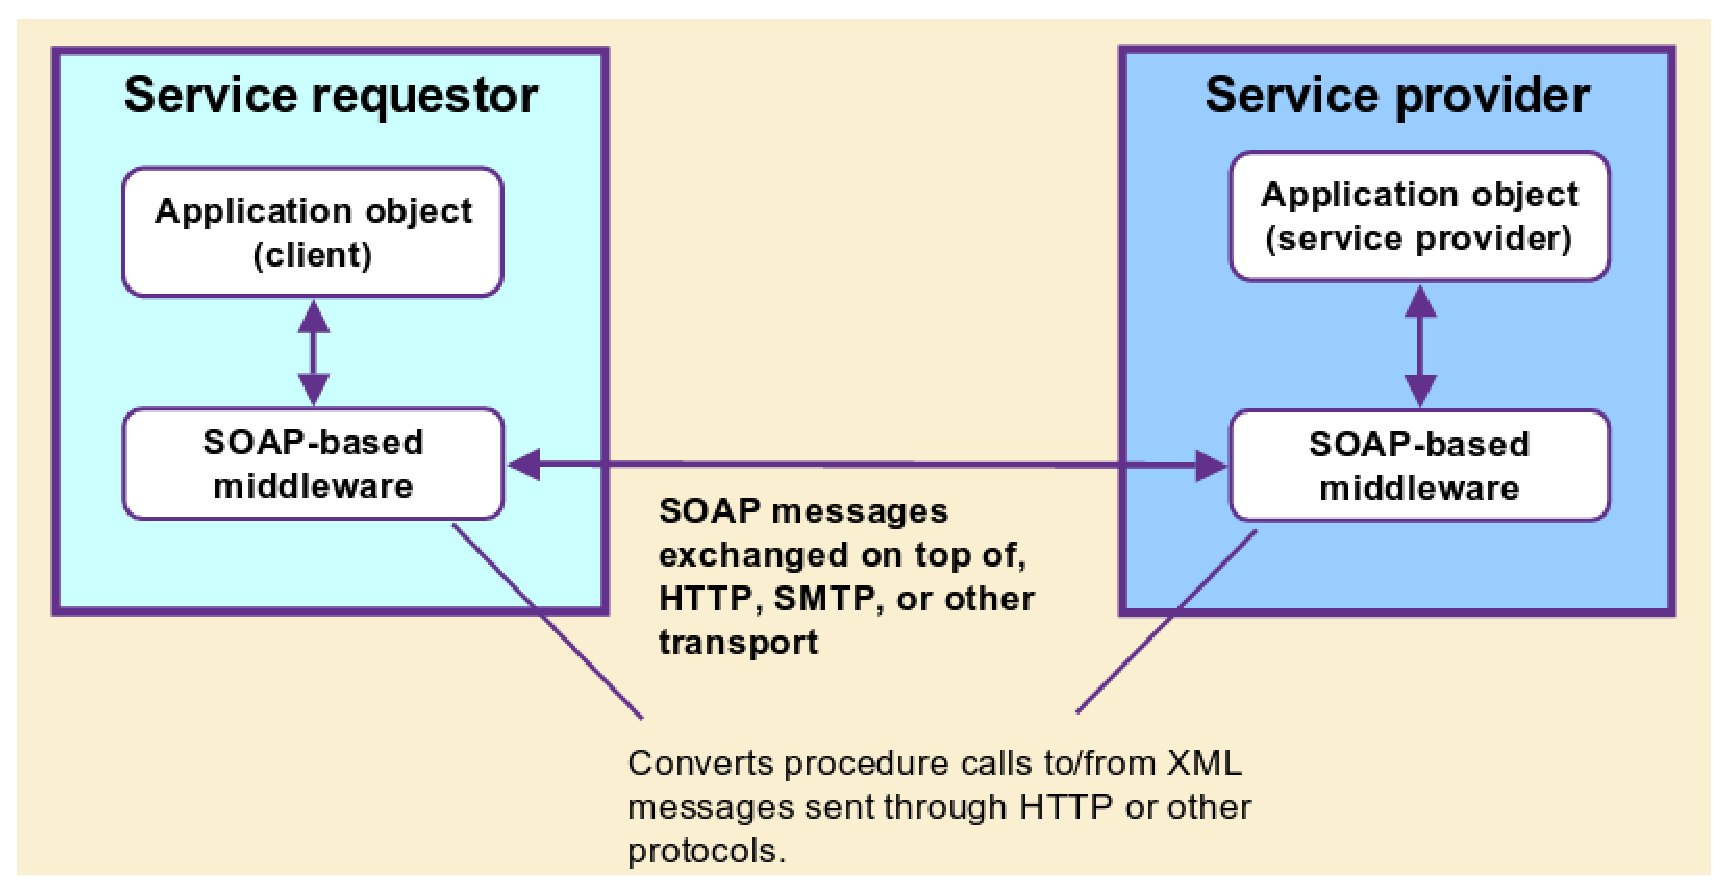
\includegraphics[width=0.8\columnwidth]{fundamentacao/webservice_soap_model_expanded} 
  \caption{SOAP no modelo Modelo de serviço web baseado em SOAP.\cite{Papazoglou_slides:2008}} 
  \label{fig:wsmodelsoap_expanded}
\end{figure}

\subsection{Serviços web RESTFul}
\label{subsec:restful}
...ver \cite{Belqasmi:2011}**

\subsection{Dispositivos como serviços web} 
\label{subsec:dispositivosweb}
//TODO ver resumo tcc odt**
Como abordado em \ref{sec:iot} um dos desafios referente a visão da IoT é sua interoperabilidade e, como possível solução se pode utilizar dos existentes protocolos web. Desta maneira os dispositivos podem interagir entre si e com outros sistemas na web.

Adotando esse padrão, os dispositivos podem ter suas propriedades disponíveis através de qualquer navegador, sem a necessidade de instalação de nenhum programa ou driver adicional, como pode ser exemplificado na Figura \ref{fig:dispnavegador}. Além disto, mashups físicos\footnotemark \footnotetext{Aplicativos criados a partir da composição de dados e serviços de dispositivos físicos com outros recursos Web.} podem ser construídos com muito menos esforço do que as existentes abordagens, quebrando drasticamente a barreira para o desenvolvimento de aplicações com dispositivos, assim então promovendo a visão da Internet das Coisas.\cite{Guinard:2009}

\begin{figure}[!htb] \centering 
  \centering
  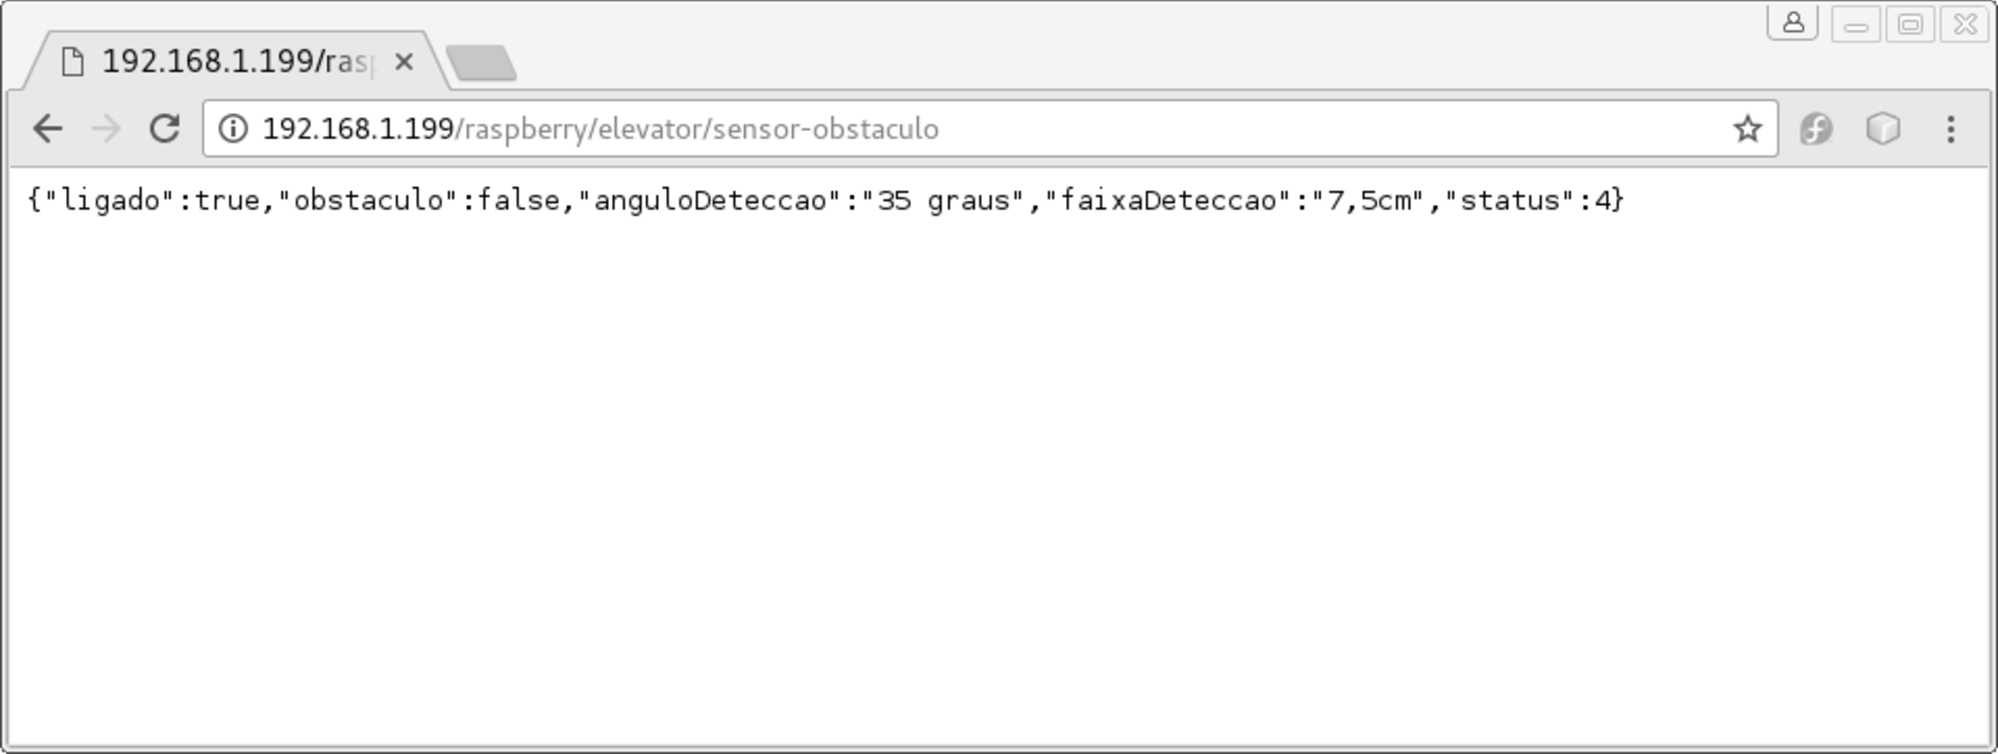
\includegraphics[width=0.8\columnwidth]{fundamentacao/elevator_sensor_example} 
  \caption{Dispositivo sensor de obstaculo do elevador disponibilizado como serviço. Faixa de detecção compatível com a largura do elevador utilizado na maquete do experimento    \ref{ch:experimento}} 
  \label{fig:dispnavegador}
\end{figure}


Nem todos os dispositivos (coisas ou objetos) possuem... TODO RESTxSOAP...

\subsection{Home network system}
\label{sec:hns}
TODO....

\section{Aprendizado supervisionado}

\subsection{Redes neurais}

\subsection{Métodos avaliativos}
pag 183 - livro data mining - parte escrita - 

\section{Interação de características}
TODO....origem...causas...etc...
\subsection{Efeitos colaterais desejáveis}
TODO....
\subsection{Efeitos colaterais indesejáveis}
Segundo \cite{Weiss:2007}o problema de efeitos colaterais indesejáveis vem sendo tratado como \textit{the feature interaction problem}.

Em \cite{Weiss}???talvez seja bom mudar esta referencia??? \textit{feature interaction} é definido como a interação entre independentes características***, as quais podem ser intencionais ou não intencionais, podendo levar a efeitos colaterais indesejáveis. Segundo \cite{Weiss:2007 } tais efeitos colaterais indesejáveis podem ser um estado inconsistente do sistema ou inconsistência de dados, tais como, um comportamento não esperado (não desejado), uma quebra de requisito de segurança, dentre outros.